
\subsection{ADC Communication}
The ADC is a MCP3008 \footnote{ \href{https://www.adafruit.com/datasheets/MCP3008.pdf}{MCP3008 Datasheet} } which communicates using SPI.
This is hence implemented in the module.
Since the ADC only allows up to 3.6MHz communication frequency, then the clock is scaled down to 3.57MHz.
The FPGA is then requesting the data from the ADC when the \textit{sample\_adc} signal is high and when the whole message is received from the ADC, it pulses a signal (\textit{spi\_data\_updated}) to notify the color detector of the new message.
The simulation of the resulting module is seen in figure \ref{fig:spi_simulation}.


\begin{figure}[H]
\centering
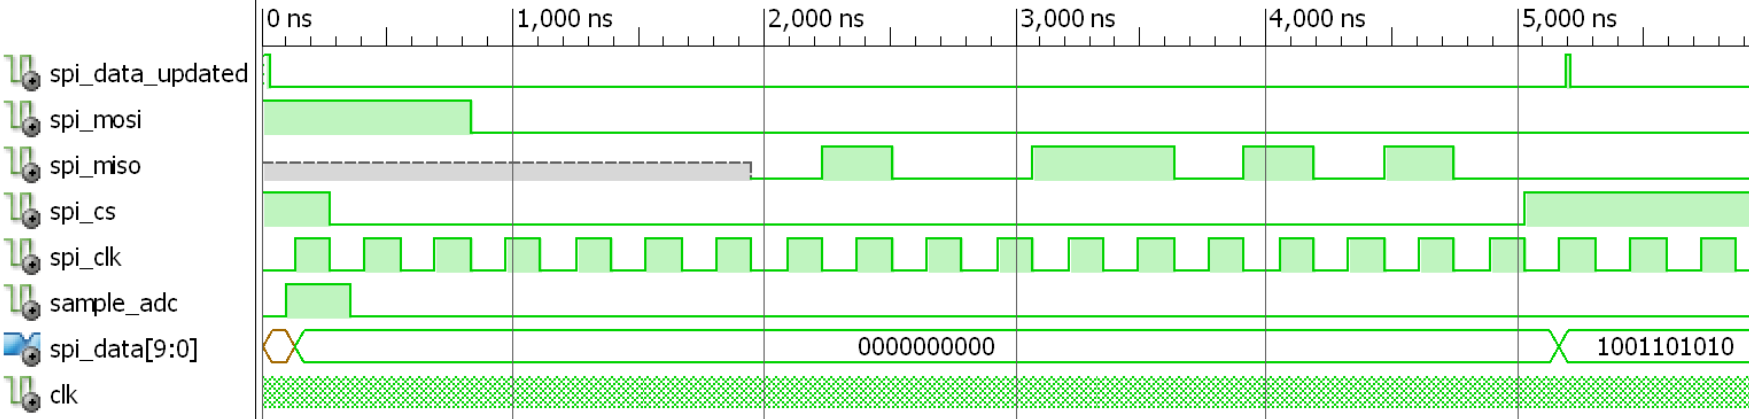
\includegraphics[width = 1 \textwidth]{simulation_SPI}
\caption{Simulation of the SPI communication with the ADC.}
\label{fig:spi_simulation}
\end{figure}

Considering figure \ref{fig:spi_simulation}, it can be found that the output gathered from the ADC is the correct one.
Furthermore the component only gets data from the ADC when requested for it.
Comparing the simulation to the specimens in the datasheet of the ADC, then the protocol is also completely followed.